\documentclass[11pt,a4paper]{article}
\usepackage[margin=22mm]{geometry}
\usepackage[T1]{fontenc}
\usepackage{lmodern}
\usepackage{graphicx,booktabs,tabularx,array,xcolor,fancyhdr,hyperref}
\definecolor{reclaim}{HTML}{245D65}
\definecolor{wash}{HTML}{ECF4F4}
\hypersetup{colorlinks=true,urlcolor=reclaim,linkcolor=reclaim}
\setlength{\parindent}{0pt}
\setlength{\parskip}{6pt}
\renewcommand{\arraystretch}{1.16}
\pagestyle{fancy}\fancyhf{}
\fancyhead[L]{\textcolor{reclaim}{\textbf{RECLAIM}}}
\fancyhead[R]{Deliverable 2 \enspace|\enspace Track A}
\fancyfoot[L]{Artificial Intelligence Semester Project}
\fancyfoot[R]{\thepage}
\setlength{\headheight}{14pt}
\newcommand{\stage}[1]{\colorbox{wash}{\parbox[c][14mm][c]{.20\linewidth}{\centering\small #1}}}
\newcommand{\commit}[1]{\href{https://github.com/Soban06/Reclaim/commit/#1}{\texttt{#1}}}
\begin{document}
{\LARGE\bfseries\color{reclaim} Reclaim}\\[3pt]
{\large Predicting return risk in e-commerce}\\[4pt]
\textbf{Deliverable 2: Model Architecture and Empirical Evaluation}\\
Track A: Application Development \hfill 10 November 2026

\begin{center}
\begin{tabularx}{\linewidth}{Xll}
\toprule Team member & Student ID & GitHub\\ \midrule
Muhammad Soban Sohail & 24L-2545 & Soban06\\
Mahad Jawad Rana & 24L-2504 & Mahad-Jawad\\
Taimur Amir & 24L-2518 & taimurrrr\\ \bottomrule
\end{tabularx}
\end{center}
\href{https://github.com/Soban06/Reclaim}{Reclaim source repository}

\section*{1. Prediction task and data}
Reclaim estimates whether an individual purchased product variant will be returned. The binary outcome is \(y=1\) for returned and \(y=0\) for kept. Product type and brand are the two predictors. Customer IDs are used for splitting. Shipping country is kept for the error audit. Average price, average discount, and return-history aggregates were excluded because their timing could not be established relative to the purchase.

The experiment uses the deterministic 100,000-event sample from Deliverable 1. About 38\% of original events lacked a required customer or product node. The source selected customers with return history, so the sample return rate is specific to this population. All three partitions come from the original training release. The official later-period test release was unused.

\section*{2. Validation strategy}
A seeded customer split (seed 42) held out 30\% of customers, then divided that group equally by customer into validation and test sets. There was zero customer overlap. Train fitted all models and preprocessing, validation selected the model and cutoff, and test was reserved for final reporting.

\begin{center}
\begin{tabularx}{\linewidth}{Xrrrr}
\toprule Partition & Purchases & Customers & Returned & Kept\\ \midrule
Train & 69,996 & 66,139 & 38,150 & 31,846\\
Validation & 14,964 & 14,173 & 8,102 & 6,862\\
Test & 15,040 & 14,173 & 8,232 & 6,808\\ \bottomrule
\end{tabularx}
\end{center}

\textbf{Main result.} Logistic regression achieved test ROC-AUC of 0.6145 versus 0.6066 for the product-type rule. At the selected cutoff of 0.42, the logistic model labeled every held-out purchase as a return.

\newpage
\section*{3. Model architecture and selection}
\begin{center}
\stage{Product type\\and brand}\(\,\to\,\)\stage{Fill missing values\\and one-hot encode}\(\,\to\,\)\stage{Logistic regression\\or decision tree}\(\,\to\,\)\stage{Return score\\and cutoff}
\end{center}
{\small\textbf{Figure 1.} The fitted preprocessing and classifier are saved as one scikit-learn pipeline. Validation chooses the classifier and cutoff before testing.}

The preprocessing fills missing values with the most frequent training value for each input and one-hot encodes the resulting categories. Unseen categories are ignored by the encoder. Logistic regression applies a sigmoid to a linear score. It minimizes binary log loss with L2 regularization using L-BFGS and a maximum of 1,000 iterations. The decision tree makes greedy Gini-impurity splits, limited by maximum depth and minimum leaf size. Neither model uses hidden layers, mini-batches or dropout.

\begin{center}
\begin{tabularx}{\linewidth}{Xlr}
\toprule Candidate & Settings & Validation ROC-AUC\\ \midrule
Logistic regression & \(C=0.1\) & \textbf{0.61564}\\
Logistic regression & \(C=1\) & 0.61561\\
Logistic regression & \(C=10\) & 0.61561\\
Decision tree & depth 3, minimum leaf 200 & 0.59306\\
Decision tree & depth 3, minimum leaf 50 & 0.59306\\
Decision tree & depth 6, minimum leaf 200 & 0.61335\\
Decision tree & depth 6, minimum leaf 50 & 0.61325\\ \bottomrule
\end{tabularx}
\end{center}

The \(C=0.1\) model had the highest validation ROC-AUC, with very small differences among the logistic settings. We searched cutoffs from 0.10 to 0.90 in steps of 0.01 for the highest validation F1, favoring the closest value to 0.50 on a tie. The selected 0.42 cutoff gave validation F1 of 0.7025.

\begin{center}
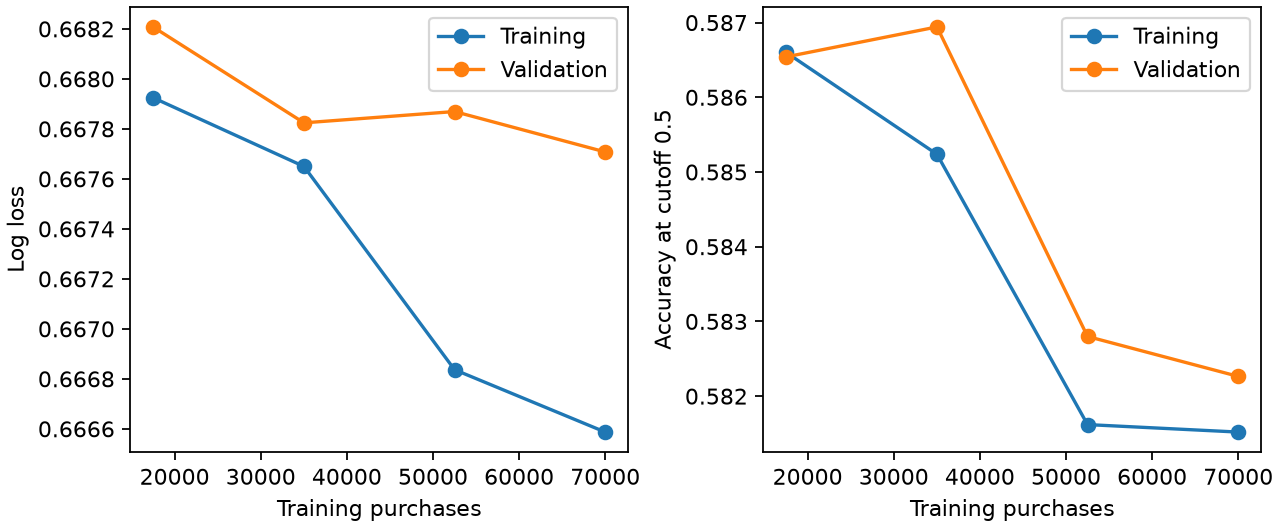
\includegraphics[width=.98\linewidth]{../figures/d2_learning_curves.png}
\end{center}
{\small\textbf{Figure 2.} Train and validation log loss and accuracy across four training-set sizes. Each run refits preprocessing on its training subset. The accuracy curves use a fixed cutoff of 0.50.}

\newpage
\section*{4. Held-out evaluation}
The majority baseline predicts a return for every purchase. The product-type rule estimates training return frequency for each type, falls back to overall training prevalence for unseen types, and uses a 0.50 cutoff. ROC-AUC evaluates ranking across thresholds. Precision measures the fraction of flagged purchases that returned, recall measures the fraction of returns caught, and F1 summarizes precision and recall. Accuracy gives the overall proportion correct.

\begin{center}
\begin{tabularx}{\linewidth}{Xrrrrr}
\toprule Method & Accuracy & Precision & Recall & F1 & ROC-AUC\\ \midrule
Majority & 0.547 & 0.547 & 1.000 & 0.707 & 0.500\\
Product-type rule & 0.580 & 0.666 & 0.466 & 0.548 & 0.607\\
Selected logistic model & 0.547 & 0.547 & 1.000 & 0.707 & 0.614\\ \bottomrule
\end{tabularx}
\end{center}

At its chosen cutoff, the model produced 8,232 true positives and 6,808 false positives, with zero true or false negatives. It therefore matched the majority baseline on every threshold-dependent metric. The product-type rule flagged fewer kept purchases (1,924 false positives) and missed 4,399 returns. The observed ranking gain over this rule is about 0.008 ROC-AUC. The experiment did not quantify uncertainty around that difference.

\begin{center}
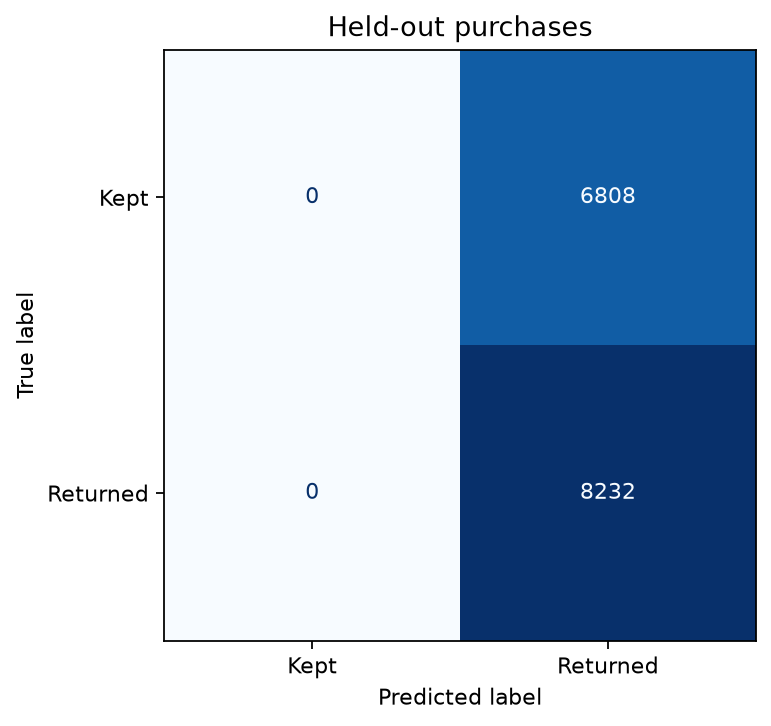
\includegraphics[width=.68\linewidth]{../figures/d2_confusion_matrix.png}
\end{center}
{\small\textbf{Figure 3.} Confusion matrix on the 15,040 held-out purchases at the validation-selected cutoff. All predictions fall in the returned column.}

\newpage
\section*{5. Bias Check and error analysis}
Across all nine anonymized shipping-country groups, the model had 100\% recall and a 100\% false-positive rate. Each group had at least 20 returned and 20 kept purchases. Equal rates here follow from predicting the same label for everyone. They provide little information about subgroup score quality or how a different cutoff would affect the groups.

\begin{center}
\begin{tabularx}{\linewidth}{Xrrrr}
\toprule Shipping group & Purchases & Returned & Kept & False positives\\ \midrule
Country E & 3,553 & 2,446 & 1,107 & 1,107\\
Country G & 8,334 & 4,189 & 4,145 & 4,145\\
Other seven groups & 3,153 & 1,597 & 1,556 & 1,556\\ \bottomrule
\end{tabularx}
\end{center}

By product type, the largest false-positive count was 3,657 for \texttt{productType\_J}, which contained 6,908 test purchases. Every kept purchase in every product type was flagged. The high count for type J therefore reflects the number of kept purchases in that group. Anonymized country codes limit interpretation, and this audit does not establish demographic fairness.

\textbf{Conclusion.} The two product fields provide some ranking signal within this sample, but the chosen cutoff is unsuitable for deciding which purchases to flag. A follow-up should set a validation objective that reflects the cost of false alarms, then use a separate later-period evaluation to assess generalization.

\section*{6. Contribution Table}
\begin{center}
\small
\begin{tabularx}{\linewidth}{@{}lXl@{}}
\toprule GitHub author & Modules and evidence added & Git commits\\ \midrule
Mahad-Jawad & Input checks, customer split, and split evidence & \commit{c95f764}, \commit{3973a72}, \commit{54510e3}\\
taimurrrr & Baselines, training and selection, and learning curves & \commit{1cf72ca}, \commit{deca2be}\\
Soban06 & Held-out evaluation, subgroup checks, and confusion matrix & \commit{fd8d720}, \commit{63d1435}\\ \bottomrule
\end{tabularx}
\end{center}
AI assistance was used to generate the supplied implementation and draft the documentation. The table records repository authorship for the listed changes.

\section*{Sources and reproducibility}
ASOS, \href{https://osf.io/c793h/}{GraphReturns dataset}, CC BY 4.0. J. McGowan et al., \href{https://arxiv.org/abs/2302.14096}{A Dataset for Learning Graph Representations to Predict Customer Returns in Fashion Retail}, 2023. Split counts, tuning settings, test metrics, and per-group results are recorded in the repository's \texttt{reports/evidence/} directory.
\end{document}


